% !TeX root = ../../ZF_bmicha_Ana.tex
\subsection{Trägheitsmoment \texorpdfstring{\hfill S.76}{S.76}}
    \subsubsection{2D}
        \textbf{Trägheitsmoment bzgl. einer Achse:}
        \begin{align*}
            I_x =& \iint_A \sigma(x,y) \cdot y^2 \, dA\\
            I_y =& \iint_A \sigma(x,y) \cdot x^2 \, dA
        \end{align*}
        \textbf{Trägheitsmoment eines Rotationskörper bzgl. seiner Achse:}
        \begin{align*}
         \textrm{explizit:} & \hspace{8pt} I_x =\frac{\pi}{2} \int y(x)^4  dx  \\
         \textrm{implizit:} & \hspace{8pt} I_x = \frac{\pi}{2} \int_{t_0}^{t_1} y(t)^4 \cdot |\dot{x}(t)| dt
         \end{align*}
        \textbf{Polares Trägheitsmom.} (bzgl. $z$-Achse/ Ursprung):
        \begin{align*}
            I_o = I_x + I_y = \iint_A \sigma(x,y) \cdot (x^2 + y^2) \, dA 
        \end{align*}
        \textit{Keine Angabe für $\sigma$: $\sigma = 1$}

    \subsubsection{3D}
        \textbf{Trägheitsmoment bzgl. Achse:}
        \begin{align*}
            I_x =& \iiint_V \rho(x,y,z) \cdot (y^2 + z^2) \, dV\\
            I_y =& \iiint_V \rho(x,y,z) \cdot (x^2 + z^2) \, dV \\
            I_z =& \iiint_V \rho(x,y,z) \cdot (x^2 + y^2) \, dV
        \end{align*}
        \textit{Keine Angabe für $\rho$: $\rho = 1$}
        \vskip5pt
    \small{Seien A bzw. B zwei disjunktive Körper (d.h. schneiden sich nicht) und a bzw. b ihr polares Trägheitsmoment um die z-Achse, so ist $I_{A \bigcup B} = a + b$ }
        
    \subsubsection{Satz von Steiner}
    \begin{minipage}{0.5\linewidth}
        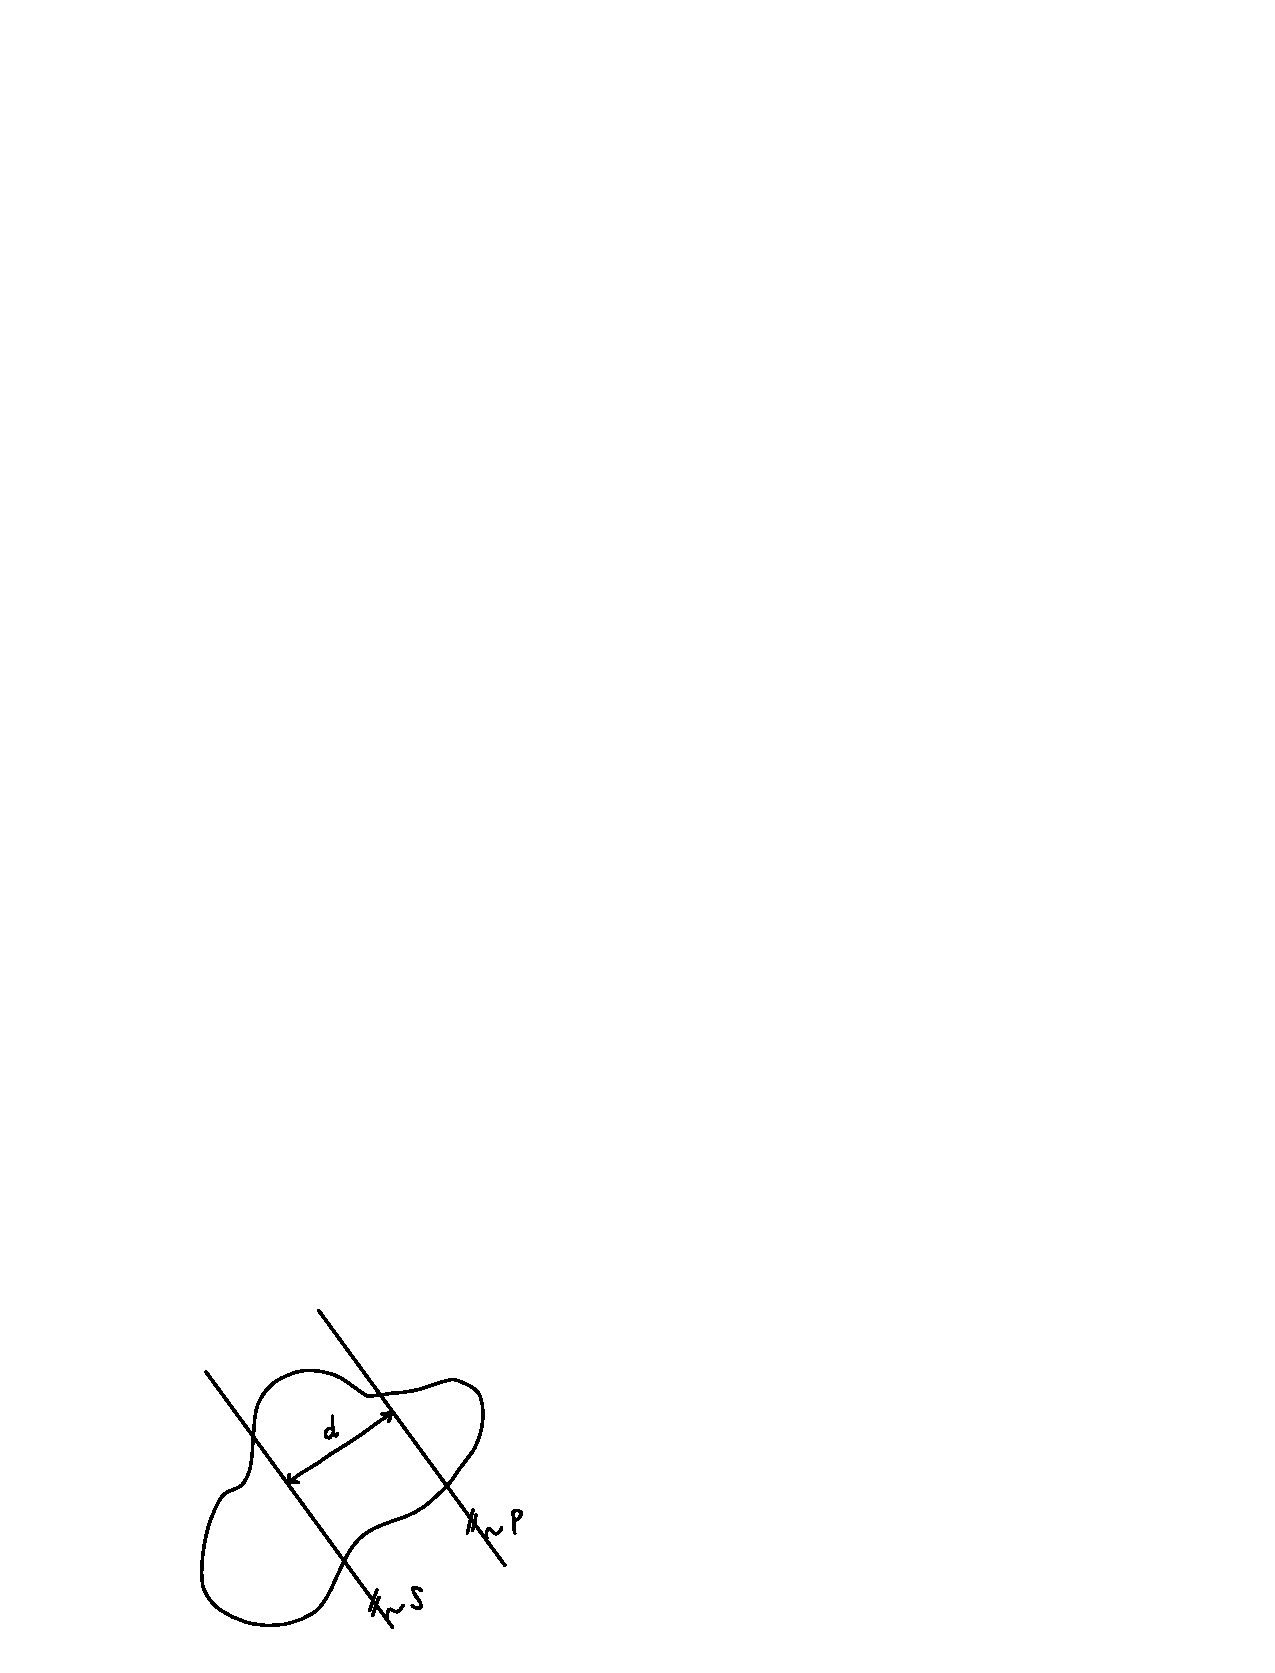
\includegraphics[width=\linewidth]{src/Mehrdimensionale-Funktionen_Integralrechnung/satz-von-steiner.pdf}
    \end{minipage}
    \hspace{0.05\linewidth}
    \begin{minipage}{0.4\linewidth}
        \begin{align*}
            I_p &=\,\, I_s + d^2 \cdot m\\
            m \vcentcolon&= Masse\\
            d \vcentcolon&= Abstand\\
        \end{align*}
    \end{minipage}